\documentclass[a4paper]{report}
\usepackage[T1]{fontenc}
\usepackage[french]{babel}
\usepackage[utf8x]{inputenc}
\usepackage{amsmath}
\usepackage{eurosym}
\usepackage{float}
\usepackage{graphicx}
\usepackage[colorinlistoftodos]{todonotes}
\usepackage{placeins}
\usepackage{verbatim}
\usepackage{fmtcount}
\usepackage[toc,page]{appendix} 

\newcommand\specification[1]{\addtocounter{cptspec}{1}\paragraph{S\thecptspec ~-  #1}~\par}
\renewcommand{\arraystretch}{1.25}
\usepackage{tabularx}

\newcounter{cptspec}
\setcounter{cptspec}{0}

 
\title{INSA de Rennes \\ Quatrième année Informatique \\ \bigskip \hrule \bigskip Rapport de Spécification \\ \bigskip Projet VaR \bigskip \hrule}

%\title{Rapport de conception : Projet POO SmallWorld}
\author{Benjamin \bsc{Bouguet} - Damien \bsc{Carduner} \\Paul \bsc{Chaignon} - Eric \bsc{Chauty} - Xavier \bsc{Fraboulet} \\ Clément \bsc{Gautrais} - Ulysse \bsc{Goarant} \\ ~~\\
Hamdi \bsc{Raissi} - Quentin \bsc{Giai Gianetto}}


\date{Novembre 2013}

\begin{document}
\maketitle
%\listoftodos

\thispagestyle{empty}
\newpage

~~
\thispagestyle{empty}
\newpage


\tableofcontents
\newpage


\chapter{Introduction}

Dans les salles de marchés, les traders achètent et vendent des actions et  obligations à longueur de journée, pour le compte de grandes banques ou investisseurs toujours à la recherche d’un maximum de profits pour des pertes minimum.
Une donnée qui peut aider les financiers à la décision, est de connaître le montant maximum qu’ils risquent de perdre pour un portefeuille d’actifs financiers donné, sur une certaine période et pour un certain niveau de risque.
En connaissant ce risque, leurs prévisions n'en seront que plus fiables et permettront peut-être d’éviter de mauvais placements. 

C’est précisément ce que notre logiciel permettra de faire : calculer la Value-at-Risk (VaR) par diverses méthodes statistiques.
Néanmoins, un unique calcul de la VaR n’est pas suffisant pour permettre de bonnes prévisions.
Pour cette raison, notre programme aura l’avantage de proposer un ensemble de tests, comparaisons, tableaux récapitulatifs et même du backtesting entre différentes méthodes statistiques.


Avec cette multitude d'outils, les financiers seront en mesure de travailler sur leurs portefeuilles aisément, au moyen d’outils de manipulations des actifs, mais aussi d’une interface simple, intuitive, ergonomique, pensée pour ne montrer que l’essentiel et être facile d’utilisation.


Ce rapport de spécification vient donner un aperçu des fonctionnalités qui seront implémentées dans notre logiciel.
Dans un premier temps, nous présenterons les spécifications fonctionnelles.
Nous indiquerons en détails quelles seront les fonctions implémentées dans le logiciel, ce qu’elles permettront de réaliser et comment elles devront être utilisées.

La seconde partie du rapport expose les spécifications techniques du logiciel.
Cela comprend les différentes techniques et technologies utilisées, ainsi qu'une première architecture globale du fonctionnement de l’application.

\chapter{Spécifications fonctionnelles}

\section{Diagramme des cas d'utilisation}

Pour présenter et définir les différentes fonctionnalités de notre programme, nous les avons modélisées au moyen de diagrammes de cas d'utitilisation.

\begin{figure}[H]
  \center
  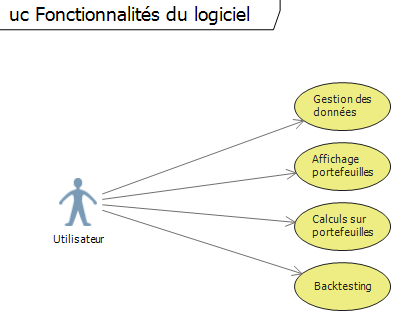
\includegraphics[width=1\textwidth]{General.png}
  \caption{Les fonctionnalités générales}
\end{figure} 

Nous avons défini quatre grandes fonctionnalités : la gestion des données, l'affichage des portefeuilles, les calculs sur les portefeuilles et le backtesting.

\subsection{Gestion des données}
\begin{figure}[H]
  \center
  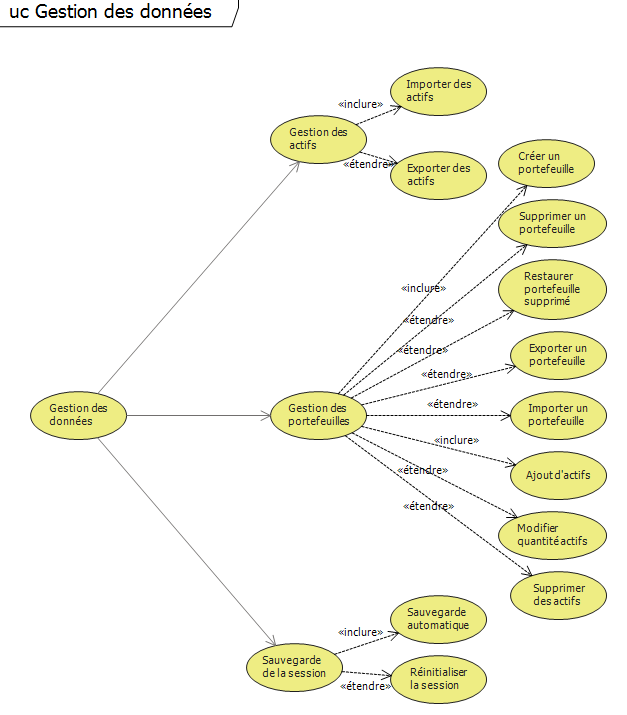
\includegraphics[width=1\textwidth]{Portefeuille.png}
  \caption{Gestion des données}
\end{figure}

La gestion des données doit permettre de manipuler à la fois les différents actifs et les portefeuilles créés.
Ces fonctionnalités contribuent à améliorer l'expérience utilisateur.
Dans cette optique, la sauvegarde de session sera une fonctionnalité appréciée par les utilisateurs.

\subsection{Affichage des portefeuilles}

\begin{figure}[H]
  \center
  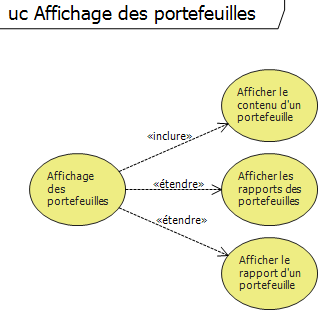
\includegraphics[scale=1]{Rapport.png}
  \caption{Affichage des portefeuilles}
\end{figure}

Pour permettre une gestion aisée des différents portefeuilles, que ce soit dans leur contenu ou dans les résultats des différents calculs, notre application conservera en mémoire tous les rapports déjà générés sur les portefeuilles, pour éviter de refaire les mêmes calculs.

\subsection{Calculs sur les portefeuilles}
\begin{figure}[H]
  \center
  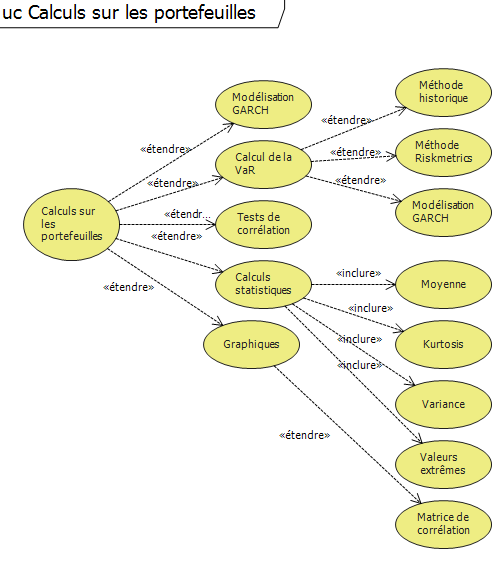
\includegraphics[width=1\textwidth]{VaR.png}
  \caption{Calculs sur les portefeuilles}
\end{figure}

Sur un ou plusieurs protefeuilles, il est possible d'effectuer différents calculs statistiques (moyenne, variance, kurtosis), calculer la VaR de différentes manières, tout en s'assurant de leur pertinence avec des tests de corrélations.
De plus, parmi les graphiques générés lors des calculs, une matrice de corrélation sera aussi construite.

\subsection{Le Backtesting}
\begin{figure}[H]
  \center
  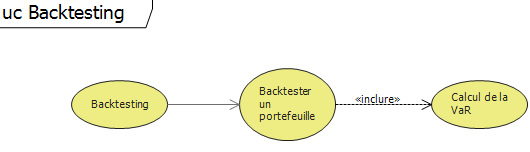
\includegraphics[width=1\textwidth]{Backtesting.png}
  \caption{Le Backtesting}
\end{figure}

Le backtesting permet d'évaluer les performances des méthodes sur un jeu de données bien particulier.
Ce n'est pas uniquement un calcul de VaR, puisque les pertes théoriques calculées sont dans un second temps comparées avec les pertes réelles historiques.
En comparant les résultats obtenus selon les méthodes de calcul de la VaR, on pourra remarquer que leurs pertinences  sont variables selon les actifs des portefeuilles, l'utilisateur pourra donc choisir quelle est celle qui convient le plus à la situation.

\FloatBarrier 





%------------------------------


\section{Spécifications}


\subsection{Gestion des données}

\subsubsection{Gestion des actifs}

\specification{Importer un ou des actifs}
Le logiciel doit permettre d'importer des actifs pour réaliser des calculs.
De plus, les fichiers CSV et Excel (format XLSX) doivent être pris en charge puisqu'ils sont très utilisés dans le domaine de la finance.
Une fois importées, les données seront stockées dans une bibliothèque regroupant tous les actifs.

\begin{table}[H]
  \begin{tabularx}{1\textwidth}{|l|X|}
    \hline
    \multicolumn{2}{|c|}{S\thecptspec - Importer un ou des actifs} \\
    \hline
    \multicolumn{2}{|l|}{Condition de déclenchement} \\
    \hline
    1- & Un utilisateur veut importer un ou des actifs \\
    \hline
    \multicolumn{2}{|l|}{Déclenchement de l’opération} \\
    \hline
    1- & L'utilisateur remplit le formulaire d'importation et valide l'opération \\
    \hline
    \multicolumn{2}{|l|}{Entrant de l’opération} \\
    \hline
    1- & Le fichier contenant les données \\
    \hline
    \multicolumn{2}{|l|}{Traitement de l’opération} \\
    \hline
    1- & Vérifie si le fichier contient des données interprétables par le logiciel\\
    2- & Identification des actifs présents dans le fichier \\
    3- & Ajout du ou des actifs dans la bibliothèque des actifs \\
    4- & Refus de l'importation si échec lors de la vérification \\
    \hline
    \multicolumn{2}{|l|}{Sortant de l’opération} \\
    \hline
    1- & Renvoi un nouveau formulaire pour importer des actifs si échec \\
    \hline
  \end{tabularx}
  \caption{S\thecptspec - Importer un ou des actifs}
\end{table}

\specification{Exporter un ou des actifs}
L’utilisateur de notre logiciel pourra aussi exporter un ou plusieurs actifs présents dans la bibliothèque sous forme de fichier CSV ou Excel.

\begin{table}[H]
  \begin{tabularx}{1\textwidth}{|l|X|}
    \hline
    \multicolumn{2}{|c|}{S\thecptspec - Exporter un ou des actifs} \\
    \hline
    \multicolumn{2}{|l|}{Condition de déclenchement} \\
    \hline
    1- & Un utilisateur veut exporter un ou des actifs \\
    \hline
    \multicolumn{2}{|l|}{Déclenchement de l’opération} \\
    \hline
    1- & L'utilisateur remplit le formulaire d'exportation et valide l'opération \\
    \hline
    \multicolumn{2}{|l|}{Entrants de l’opération} \\
    \hline
    1- & Le type de fichier de sortie \\
    2- & L'emplacement où enregistrer le fichier \\
    3- & La liste des actifs à exporter \\
    \hline
    \multicolumn{2}{|l|}{Traitement de l’opération} \\
    \hline
    1- & Vérifie la présence des actifs dans la bibliothèque \\
    2- & Construit un fichier du type demandé comprenant les actifs \\
    3- & Enregistre le fichier créé à l'emplacement choisi par l'utilisateur \\
    \hline
    \multicolumn{2}{|l|}{Sortant de l’opération} \\
    \hline
  \end{tabularx}
  \caption{S\thecptspec - Exporter un ou des actifs}
\end{table}


\subsubsection{Gestion des portefeuilles}

La gestion d’un portefeuille est l’un des enjeux importants de notre logiciel.
En effet, l’utilisateur sera amené à manipuler très régulièrement les fonctionnalités de la gestion de portefeuille.
C’est pour cela qu’il faut que la gestion du portefeuille soit la plus simple possible pour ne pas dissuader l’utilisateur d’utiliser les différentes fonctionnalités.
La manipulation de portefeuilles volumineux en termes d'actifs doit être gérée tout aussi facilement que la manipulation des plus petits.

\specification{Créer un portefeuille}

À partir de l’ensemble des données, la première action sera de créer un portefeuille d’actifs.
Pour cela une option dans le menu fichier permettra à l’utilisateur de créer un nouveau portefeuille d’actifs.
Un bouton dans la barre de raccourci permettra également sa création.

\begin{table}[H]
  \begin{tabularx}{1\textwidth}{|l|X|}
    \hline
    \multicolumn{2}{|c|}{S\thecptspec - Créer un portefeuille} \\
    \hline
    \multicolumn{2}{|l|}{Condition de déclenchement} \\
    \hline
    1- & Un utilisateur souhaite créer un portefeuille \\
    \hline
    \multicolumn{2}{|l|}{Déclenchement de l’opération} \\
    \hline
    1- & L'utilisateur remplit le formulaire puis valide l'opération \\
    \hline
    \multicolumn{2}{|l|}{Entrants de l’opération} \\
    \hline
    1- & Le nom du portefeuille créé \\
    2- & La liste des données à insérer dans le portefeuille \\
    \hline
    \multicolumn{2}{|l|}{Traitement de l’opération} \\
    \hline
    1- & Vérifie si le portefeuille existe \\
    2- & Ajoute le portefeuille à la liste des existants \\
    \hline
    \multicolumn{2}{|l|}{Sortants de l’opération} \\
    \hline
    1- & Message de confirmation si l'opération s'est bien passée \\
    2- & Message d'erreur en cas d'échec \\
    \hline
  \end{tabularx}
  \caption{S\thecptspec - Créer un portefeuille}
\end{table}

\specification{Supprimer un portefeuille}

La suppression des portefeuilles permet à l'utilisateur d'avoir un moyen simple de tenir à jour la liste des actifs financiers qu'il possède.

\begin{table}[H]
  \begin{tabularx}{1\textwidth}{|l|X|}
    \hline
    \multicolumn{2}{|c|}{S\thecptspec - Supprimer un portefeuille} \\
    \hline
    \multicolumn{2}{|l|}{Condition de déclenchement} \\
    \hline
    1- & Un utilisateur souhaite supprimer un portefeuille \\
    \hline
    \multicolumn{2}{|l|}{Déclenchement de l’opération} \\
    \hline
    1- & L'utilisateur indique le nom du portefeuille à supprimer et valide l'opération\\
    \hline
    \multicolumn{2}{|l|}{Entrants de l’opération} \\
    \hline
    1- & Le portefeuille à supprimer \\
    \hline
    \multicolumn{2}{|l|}{Traitement de l’opération} \\
    \hline
    1- & Vérifie si le portefeuille existe \\
    2- & Supprime le portefeuille de la liste des portefeuilles \\
    \hline
    \multicolumn{2}{|l|}{Sortant de l’opération} \\
    \hline
    1- & Message de confirmation si l'opération s'est bien passée \\
    2- & Message d'erreur en cas d'échec \\
    \hline
  \end{tabularx}
  \caption{S\thecptspec - Suppression des portefeuilles}
\end{table}

\specification{Restaurer un portefeuille supprimé}

Comme la suppression d'un portefeuille ne supprime pas le fichier créé lors de la sauvegarde, si l'utilisateur regrette d'en avoir supprimé un, il pourra simplement le restaurer.
\begin{table}[H]
  \begin{tabularx}{1\textwidth}{|l|X|}
    \hline
    \multicolumn{2}{|c|}{S\thecptspec - Restaurer un portefeuille supprimé} \\
    \hline
    \multicolumn{2}{|l|}{Condition de déclenchement} \\
    \hline
    1- & Un utilisateur souhaite restaurer un portefeuille supprimé\\
    \hline
    \multicolumn{2}{|l|}{Déclenchement de l’opération} \\
    \hline
    1- & L'utilisateur indique le nom du portefeuille à restaurer et valide l'opération\\
    \hline
    \multicolumn{2}{|l|}{Entrants de l’opération} \\
    \hline
    1- & Le portefeuille à restaurer \\
    \hline
    \multicolumn{2}{|l|}{Traitement de l’opération} \\
    \hline
    1- & Vérifie si le portefeuille existe \\
    2- & Ajoute le portefeuille à la liste des portefeuilles \\
    \hline
    \multicolumn{2}{|l|}{Sortant de l’opération} \\
    \hline
    1- & Message de confirmation si l'opération s'est bien passée \\
    2- & Message d'erreur en cas d'échec \\
    \hline
  \end{tabularx}
  \caption{S\thecptspec - Restauration d'un portefeuille}
\end{table}


\specification{Ajouter des actifs à un portefeuille}
Les portefeuilles sont constitués d'actifs.
Manipuler des portefeuilles implique donc de pouvoir ajouter des actifs à un portefeuille.

\begin{table}[H]
  \begin{tabularx}{1\textwidth}{|l|X|}
    \hline
    \multicolumn{2}{|c|}{S\thecptspec - Ajouter des actifs à un portefeuille} \\
    \hline
    \multicolumn{2}{|l|}{Condition de déclenchement} \\
    \hline
    1- & Un utilisateur souhaite ajouter un actif à un portefeuille \\
    \hline
    \multicolumn{2}{|l|}{Déclenchement de l’opération} \\
    \hline
    1- & L'utilisateur ajoute un actif provenant de la liste des actifs présents dans la liste des données \\
    \hline
    \multicolumn{2}{|l|}{Entrants de l’opération} \\
    \hline
    1- & Le nom de l'actif à ajouter \\
    2- & La quantité de cet actif à ajouter \\
    \hline
    \multicolumn{2}{|l|}{Traitement de l’opération} \\
    \hline
    1- & Vérifie si l'actif est déjà présent dans le portefeuille \\
    2- & Ajoute l'actif au portefeuille \\
    \hline
    \multicolumn{2}{|l|}{Sortant de l’opération} \\
    \hline
  \end{tabularx}
  \caption{S\thecptspec - Ajouter des actifs à un portefeuille}
\end{table}

\specification{Modifier la quantité d'actifs dans un portefeuille}
La quantité d'un actif donné est une donnée essentielle dans la constitution d'un portefeuille.
Pouvoir agir directement sur ce paramètre est donc essentiel pour un utilisateur.

\begin{table}[H]
  \begin{tabularx}{1\textwidth}{|l|X|}
    \hline
    \multicolumn{2}{|c|}{S\thecptspec - Modifier la quantité d'actifs dans un portefeuille} \\
    \hline
    \multicolumn{2}{|l|}{Condition de déclenchement} \\
    \hline
    1- & Un utilisateur souhaite modifier dans son portefeuille la quantité d'un actif donné \\
    \hline
    \multicolumn{2}{|l|}{Déclenchement de l’opération} \\
    \hline
    1- & L'utilisateur remplit le formulaire permettant de modifier la quantité d'actif \\
    \hline
    \multicolumn{2}{|l|}{Entrants de l’opération} \\
    \hline
    1- & Le portefeuille dans lequel se situe l'actif  \\
    2- & Le nom de l'actif dont l'utilisateur souhaite modifier la quantité \\
    3- & La nouvelle quantité de l'actif dans le portefeuille \\
    \hline
    \multicolumn{2}{|l|}{Traitement de l’opération} \\
    \hline
    1- & Vérifie si le portefeuille existe \\
    2- & Vérifie si l'actif appartient au portefeuille \\
    3- & Modifie la quantité d'actif dans le portefeuille \\
    \hline
    \multicolumn{2}{|l|}{Sortant de l’opération} \\
    \hline
  \end{tabularx}
  \caption{S\thecptspec - Modifier la quantité d'actifs dans un portefeuille}
\end{table}

\specification{Supprimer des actifs dans un portefeuille}
Toujours dans l'idée de permettre à l'utilisateur de gérer au mieux ses portefeuilles, la fonctionnalité de supprimer un actif au portefeuille sera naturellement implémentée au projet.
\begin{table}[H]
  \begin{tabularx}{1\textwidth}{|l|X|}
    \hline
    \multicolumn{2}{|c|}{S\thecptspec - Supprimer des actifs dans un portefeuille} \\
    \hline
    \multicolumn{2}{|l|}{Condition de déclenchement} \\
    \hline
    1- & Un utilisateur souhaite supprimer un actif dans un portefeuille \\
    \hline
    \multicolumn{2}{|l|}{Déclenchement de l’opération} \\
    \hline
    1- & L'utilisateur remplit le formulaire de suppression d'un actif dans un portefeuille \\
    \hline
    \multicolumn{2}{|l|}{Entrants de l’opération} \\
    \hline
    1- & Le portefeuille dans lequel l'actif à supprimer se situe\\
    2- & Nom de l'actif que l'utilisateur souhaite supprimer \\
    \hline
    \multicolumn{2}{|l|}{Traitement de l’opération} \\
    \hline
    1- & Vérifier si le portefeuille existe \\
    2- & Supprimer l'actif de la liste des actifs associés au portefeuille\\
    \hline
    \multicolumn{2}{|l|}{Sortant de l’opération} \\
    \hline
  \end{tabularx}
  \caption{S\thecptspec - Supprimer des actifs dans un portefeuille}
\end{table}

\specification{Exporter un portefeuille}
L’exportation sera proposée afin de permettre de partager un même portefeuille avec plusieurs utilisateurs du logiciel.
Le fichier créé à l’issue de cette opération contiendra pour chaque actif : sa valeur en fonction du temps ainsi que la quantité présente dans le portefeuille.

\begin{table}[H]
  \begin{tabularx}{1\textwidth}{|l|X|}
    \hline
    \multicolumn{2}{|c|}{S\thecptspec - Exporter un portefeuille} \\
    \hline
    \multicolumn{2}{|l|}{Condition de déclenchement} \\
    \hline
    1- & Un utilisateur veut exporter un portefeuille \\
    \hline
    \multicolumn{2}{|l|}{Déclenchement de l’opération} \\
    \hline
    1- & L'utilisateur remplit le formulaire d'exportation et valide l'opération \\
    \hline
    \multicolumn{2}{|l|}{Entrants de l’opération} \\
    \hline
    1- & Le portefeuille à exporter \\
    2- & Emplacement où enregistrer le fichier \\
    \hline
    \multicolumn{2}{|l|}{Traitement de l’opération} \\
    \hline
    1- & Vérifie si le portefeuille existe \\
    2- & Enregistre le portefeuille à l'emplacement choisi par l'utilisateur \\
    \hline
    \multicolumn{2}{|l|}{Sortant de l’opération} \\
    \hline
  \end{tabularx}
  \caption{S\thecptspec - Exporter un portefeuille}
\end{table}


\specification{Importer un portefeuille}
Puisque le logiciel proposera de créer des portefeuilles et de les exporter, il permettra aussi de les importer.
Pour cela, l’utilisateur devra sélectionner le fichier contenant le portefeuille grâce à un explorateur de fichiers.
Après importation par le logiciel, celui-ci sera présent dans la liste des portefeuilles : l’utilisateur pourra alors réaliser des calculs dessus.
Les actifs présents seront aussi importés dans la bibliothèque afin de permettre à l’utilisateur de les réutiliser dans un autre portefeuille.

\begin{table}[H]
  \begin{tabularx}{1\textwidth}{|l|X|}
    \hline
    \multicolumn{2}{|c|}{S\thecptspec - Importer un portefeuille} \\
    \hline
    \multicolumn{2}{|l|}{Condition de déclenchement} \\
    \hline
    1- & Un utilisateur veut importer un portefeuille \\
    \hline
    \multicolumn{2}{|l|}{Déclenchement de l’opération} \\
    \hline
    1- & L'utilisateur remplit le formulaire d'importation et valide l'opération \\
    \hline
    \multicolumn{2}{|l|}{Entrants de l’opération} \\
    \hline
    1- & Le fichier contenant le portefeuille \\
    \hline
    \multicolumn{2}{|l|}{Traitement de l’opération} \\
    \hline
    1- & Vérifie si le fichier contient un portefeuille \\
    2- & Ajout du portefeuille dans le logiciel \\
    3- & Ajout des actifs du portefeuille dans la bibliothèque \\
    4- & Refus de l'importation si échec lors de la vérification \\
    \hline
    \multicolumn{2}{|l|}{Sortant de l’opération} \\
    \hline
    1- & Renvoi un nouveau formulaire pour importer un portefeuille si échec \\
    \hline
  \end{tabularx}
  \caption{S\thecptspec - Importer un portefeuille}
\end{table}

\subsubsection{Sauvegarde de la session}
\specification{Sauvegarder automatiquement la session en cours}

Le logiciel proposera une option dans l’interface pour enregistrer la session en cours.
Elle sera aussi proposée à la fermeture du logiciel.
L’ensemble des portefeuilles, des calculs effectués et la bibliothèque d’actifs seront alors sauvegardés sur le disque dur.
Ainsi, lorsque l’utilisateur relancera le logiciel, ses données seront déjà présentes : il ne sera donc pas nécessaire de ré-importer les actifs et les portefeuilles à chaque lancement du logiciel.


\specification{Réinitialiser la session}
Le logiciel permettra de réinitialiser la session en cours.
C'est à dire qu'il permettra de supprimer la bibliothèque d'actifs, les portefeuilles constitués et les calculs effectués.






\FloatBarrier 
%------------------------------


\subsection{Affichage des portefeuilles}

\specification{Afficher le contenu d'un portefeuille}
L’affichage des données brutes d’un portefeuille se fera dans un tableau de données affiché dans l’onglet Données.
Ce tableau listera les actifs du portefeuille.
\begin{table}[H]
  \begin{tabularx}{1\textwidth}{|l|X|}
    \hline
    \multicolumn{2}{|c|}{S\thecptspec - Afficher le contenu d'un portefeuille} \\
    \hline
    \multicolumn{2}{|l|}{Condition de déclenchement} \\
    \hline
    1- & L'utilisateur veut afficher les données d'un portefeuille \\
    \hline
    \multicolumn{2}{|l|}{Déclenchement de l’opération} \\
    \hline
    1- & L'utilisateur sélectionne un portefeuille \\
    2- & L'utilisateur sélectionne l'onglet de données \\
    \hline
    \multicolumn{2}{|l|}{Entrants de l’opération} \\
    \hline
    1- & Le portefeuille que l'on souhaite afficher\\
    \hline
    \multicolumn{2}{|l|}{Traitement de l’opération} \\
    \hline
    1- & Vérifier si le portefeuille existe \\
    2- & Charger les données dans le tableau \\
    \hline
    \multicolumn{2}{|l|}{Sortant de l’opération} \\
    \hline
  \end{tabularx}
  \caption{S\thecptspec - Afficher le contenu d'un portefeuille}
\end{table}

\specification{Afficher les rapports d'un portefeuille}
Lorsque l'utilisateur réalise un calcul sur un portefeuille, un rapport est généré afin de garder une trace.
Ces rapports seront mis dans l’onglet Résultats.
Les différents types de rapport (graphique ou textuel) s’afficheront sous forme de vignettes.

\begin{table}[H]
  \begin{tabularx}{1\textwidth}{|l|X|}
    \hline
    \multicolumn{2}{|c|}{S\thecptspec - Afficher les rapports d'un portefeuille} \\
    \hline
    \multicolumn{2}{|l|}{Condition de déclenchement} \\
    \hline
    1- & L'utilisateur veut afficher les rapports d'un portefeuille \\
    \hline
    \multicolumn{2}{|l|}{Déclenchement de l’opération} \\
    \hline
    1- & L'utilisateur sélectionne un portefeuille \\
    2- & L'utilisateur sélectionne l'onglet de résultats \\
    \hline
    \multicolumn{2}{|l|}{Entrants de l’opération} \\
    \hline
    1- & Le portefeuille sélectionné \\
    \hline
    \multicolumn{2}{|l|}{Traitement de l’opération} \\
    \hline
    1- & Vérifier si le portefeuille existe \\
    2- & Charger la liste des rapports du portefeuille \\
    3- & Pour chaque rapport : afficher une vignette en fonction du type de rapport (textuel, histogramme, etc.) \\
    \hline
    \multicolumn{2}{|l|}{Sortant de l’opération} \\
    \hline
  \end{tabularx}
  \caption{S\thecptspec - Afficher les rapports d'un portefeuille}
\end{table}




\specification{Afficher un rapport d'un portefeuille}
La sélection d'une vignette affichera la rapport ou le graphique dans l'onglet.

\begin{table}[H]
  \begin{tabularx}{1\textwidth}{|l|X|}
    \hline
    \multicolumn{2}{|c|}{S\thecptspec - Afficher un rapport d'un portefeuille} \\
    \hline
    \multicolumn{2}{|l|}{Condition de déclenchement} \\
    \hline
    1- & L'utilisateur veut afficher l'un des rapports d'un portefeuille \\
    \hline
    \multicolumn{2}{|l|}{Déclenchement de l’opération} \\
    \hline
    1- & L'utilisateur sélectionne un portefeuille \\
    2- & L'utilisateur sélectionne l'onglet Résultat \\
    3- & L'utilisateur sélectionne un rapport dans la liste des vignettes \\
    \hline
    \multicolumn{2}{|l|}{Entrants de l’opération} \\
    \hline
    1- & Le portefeuille sélectionné \\
    2- & Le rapport sélectionné \\
    \hline
    \multicolumn{2}{|l|}{Traitement de l’opération} \\
    \hline
    1- & Vérifier si le portefeuille existe \\
    2- & Vérifier si le rapport existe \\
    3- & Afficher le rapport en fonction de son type \\
    \hline
    \multicolumn{2}{|l|}{Sortant de l’opération} \\
    \hline
  \end{tabularx}
  \caption{S\thecptspec - Afficher un rapport d'un portefeuille}
\end{table}





\FloatBarrier 
%------------------------------



\subsection{Calculs sur les portefeuilles}

\subsubsection{Calcul de la VaR}

Toutes les actions utilisateurs présentées dans la suite ont lieu sur un portefeuille.
Elles se feront donc sur le portefeuille courant lorsqu'elles auront été lancées depuis le menu.
Elles pourront aussi être lancées en effectuant un clic droit sur le portefeuille ciblé.


\specification{Tester la validité du modèle par des tests de corrélation}
L'utilisateur pourra tester la validité d'une éventuelle modélisation GARCH sur son portefeuille.
Pour cela, il disposera du choix entre deux tests : corrélation simple et corrélation à l'ordre deux.
Ces deux tests peuvent être lancés depuis le menu mais seront aussi proposés précédemment au calcul d'une modélisation GARCH.

\begin{table}[H]
  \begin{tabularx}{1\textwidth}{|l|X|}
    \hline
    \multicolumn{2}{|c|}{S\thecptspec - Tester la validité du modèle par des tests de corrélation} \\
    \hline
    \multicolumn{2}{|l|}{Condition de déclenchement} \\
    \hline
    1- & L'utilisateur veut vérifier la validité d'une modélisation GARCH \\
    \hline
    \multicolumn{2}{|l|}{Déclenchement de l’opération} \\
    \hline
    1- & L'utilisateur fixe les entrants et valide \\
    \hline
    \multicolumn{2}{|l|}{Entrants de l’opération} \\
    \hline
    1- & Portefeuille sur lequel va se faire la modélisation \\
    2- & Type de corrélation \\
    \hline
    \multicolumn{2}{|l|}{Traitement de l’opération} \\
    \hline
    1- & Calcul de la corrélation \\
    \hline
    \multicolumn{2}{|l|}{Sortant de l’opération} \\
    \hline
    1- & Validité de la modélisation GARCH \\
    \hline
  \end{tabularx}
  \caption{S\thecptspec - Tester la validité du modèle par des tests de corrélation}
\end{table}

\specification{Effectuer la modélisation GARCH}
Une des trois méthodes\footnote{Les trois méthodes sont la méthode historique, la méthode avec modélisation GARCH et la méthode RiskMetrics} permettant de calculer la Value-at-Risk s'appuie sur une modélisation GARCH des données.
Parce que le calcul de cette modélisation peut prendre un moment, nous permettrons à l'utilisateur de calculer la modélisation indépendemment de la VaR.

L'opération génèrera un rapport associé au portefeuille détaillant les résultats.
Le calcul pourra être mis en arrière-plan.
L'utilisateur sera notifié de la fin du calcul.

\begin{table}[H]
  \begin{tabularx}{1\textwidth}{|l|X|}
    \hline
    \multicolumn{2}{|c|}{S\thecptspec - Effectuer la modélisation GARCH} \\
    \hline
    \multicolumn{2}{|l|}{Condition de déclenchement} \\
    \hline
    1- & L'utilisateur veut une modélisation de GARCH de ses données \\
    \hline
    \multicolumn{2}{|l|}{Déclenchement de l’opération} \\
    \hline
    1- & L'utilisateur demande une modélisation GARCH des données \\
    \hline
    \multicolumn{2}{|l|}{Entrant de l’opération} \\
    \hline
    1- & Portefeuille sélectionné pour la modélisation \\
    2- & La période sur laquelle l'utilisateur veut effectuer la modélisation \\
    \hline
    \multicolumn{2}{|l|}{Traitement de l’opération} \\
    \hline
    1- & Calcul de la modélisation GARCH \\
    2- & Génération d'un rapport de modélisation \\
    \hline
    \multicolumn{2}{|l|}{Sortant de l’opération} \\
    \hline
    1- & Notification à la fin du calcul \\
    \hline
  \end{tabularx}
  \caption{S\thecptspec - Effectuer la modélisation GARCH}
\end{table}


\specification{Calculer la Value-at-Risk}

Comme dit précedemment, le calcul de la VaR peut être effectué selon trois méthodes.
L'utilisateur pourra, via un formulaire simple, fixer les paramètres et choisir la méthode de calcul. Si ce dernier choisit d'effectuer le calcul depuis une modélisation GARCH, la sélection de la modélisation sera aussi demandée.
A ce moment, si aucune modélistion n'a encore été calculée, l'utilisateur pourra choisir d'en effectuer une nouvelle.
Les paramètres en entrée pour la modélisation seront alors demandés précédemment au calcul de la VaR.

L'opération génèrera un rapport détaillant les résultats.
Comme le calcul peut prendre un moment, il pourra être mis en arrière-plan.
A la fin de l'opération, la VaR sera affichée.


\begin{table}[H]
  \begin{tabularx}{1\textwidth}{|l|X|}
    \hline
    \multicolumn{2}{|c|}{S\thecptspec - Calculer la Value-at-Risk} \\
    \hline
    \multicolumn{2}{|l|}{Condition de déclenchement} \\
    \hline
    1- & L'utilisateur souhaite calculer la Value-at-Risk de son portefeuille \\
    \hline
    \multicolumn{2}{|l|}{Déclenchement de l’opération} \\
    \hline
    1- & L'utilisateur fixe les entrants et valide \\
    \hline
    \multicolumn{2}{|l|}{Entrants de l’opération} \\
    \hline
    1- & Méthode de calcul \\
    2- & Niveau de risque \\
    3- & Horizon de la VaR \\
    4- & Dernière date prise en compte \\
    5- & Modélisation GARCH dans le cas d'un choix de méthode GARCH \\
    \hline
    \multicolumn{2}{|l|}{Traitement de l’opération} \\
    \hline
    1- & Vérification de la validité du niveau de risque \\
    2- & Calcul de la Value-at-Risk suivant la méthode choisie \\
    3- & Génération du rapport détaillant les résultats \\
    \hline
    \multicolumn{2}{|l|}{Sortants de l’opération} \\
    \hline
    1- & Renvoi d'un nouveau formulaire de calcul de la VaR si le niveau de risque n'est pas valide \\
    2- & Notification à la fin du calcul \\
    \hline
  \end{tabularx}
  \caption{S\thecptspec - Calculer la Value-at-Risk}
\end{table}




\subsubsection{Calculs statistiques sur les portefeuilles}

\specification{Effectuer des calculs statistiques standards sur un portefeuille}
Des calculs statistiques standards pourront être effectués sur les données et seront compilés dans un format textuel.
Ce rapport contiendra le calcul de la moyenne, la variance, le kurtosis et les valeurs extrêmes de l’ensemble des données.


\begin{table}[H]
  \begin{tabularx}{1\textwidth}{|l|X|}
    \hline
    \multicolumn{2}{|c|}{S\thecptspec - Effectuer des calculs statistiques standards sur un portefeuille} \\
    \hline
    \multicolumn{2}{|l|}{Condition de déclenchement} \\
    \hline
    1- & L'utilisateur veut générer un rapport sur les statistiques générales du portefeuille \\
    \hline
    \multicolumn{2}{|l|}{Déclenchement de l’opération} \\
    \hline
    1- & L'utilisateur sélectionne un portefeuille \\
    2- & L'utilisateur clique sur le bouton "Générer rapport statistique" \\
    \hline
    \multicolumn{2}{|l|}{Entrants de l’opération} \\
    \hline
    1- & Le portefeuille sélectionné \\
    \hline
    \multicolumn{2}{|l|}{Traitement de l’opération} \\
    \hline
    1- & Vérifier si le portefeuille existe \\
    2- & Calculer la moyenne \\
    3- & Calculer la variance \\
    4- & Calculer le kurtosis \\
    5- & Calculer les valeurs extrêmes \\
    \hline
    \multicolumn{2}{|l|}{Sortant de l’opération} \\
    \hline
    1- & Le rapport de statistique \\
    \hline
  \end{tabularx}
  \caption{S\thecptspec - Effectuer des calculs statistiques standards sur un portefeuille}
\end{table}


\subsubsection{Graphiques}
En plus des graphiques généraux présentés précédemment, notre client souhaite avoir la possibilité de générer une autre information graphique : une matrice de corrélation.

La matrice de corrélation représente la corrélation entre les différents types d’indices.
L’idée derrière cette matrice est que lorsque le marché est en situation “normale”, les investissements sont relativement indépendants.
En revanche, lorsque qu’une crise touche les marchés financiers, tous les indices ont tendance à baisser et ils sont donc plus fortement corrélés (à la baisse).
Le calcul de la matrice de corrélation est donc plutôt lié à un portefeuille composé d’actifs variés, afin de vérifier que les actifs n'ont pas tendance à être plus corrélés.
Par ailleurs, ce calcul de la matrice de corrélation devra être répété plusieurs fois sur une période déterminée par l’utilisateur (tous les mois, semaines...).
En effet, la matrice de corrélation seule apporte une information limitée tandis que l’évolution de cette matrice au cours du temps permet de mieux repérer les tendances du marché.

\specification{Générer la matrice de corrélation}

Pour l’utilisateur, le calcul de la matrice de corrélation sera une action réalisable sur un portefeuille.
Le calcul inclura donc la corrélation entre tous les actifs du portefeuille.

\begin{table}[H]
  \begin{tabularx}{1\textwidth}{|l|X|}
    \hline
    \multicolumn{2}{|c|}{S\thecptspec - Générer la matrice de corrélation} \\
    \hline
    \multicolumn{2}{|l|}{Condition de déclenchement} \\
    \hline
    1- & L'utilisateur souhaite calculer la matrice de corrélation sur un portefeuille \\
    \hline
    \multicolumn{2}{|l|}{Déclenchement de l’opération} \\
    \hline
    1- & L'utilisateur spécifie les paramètres du calcul et valide l'opération \\
    \hline
    \multicolumn{2}{|l|}{Entrants de l’opération} \\
    \hline
    1- & Le portefeuille sur lequel sera effectué le calcul \\
    2- & La période sur laquelle on calcule la matrice \\
    3a- & Le nombre de matrices de corrélation que l'on souhaite générer \\
    3b- & La période utilisée pour calculer les matrices \\
    \hline
    \multicolumn{2}{|l|}{Traitement de l’opération} \\
    \hline
    1- & Vérification que le portefeuille existe \\
    2- & Déterminer la période utilisée pour le calcul de chaque matrice de corrélation \\
    3- & Calculer chaque matrice de corrélation entre tous les actifs du portefeuille\\
    4- & Générer la représentation graphique de chaque matrice calculée\\
    5- & Créer un rapport contenant toutes les rerésentations graphiques\\
    6- & Placer le rapport dans la zone des rapports liés au portefeuille\\
    \hline
    \multicolumn{2}{|l|}{Sortant de l’opération} \\
    \hline
  \end{tabularx}
  \caption{S\thecptspec - Générer la matrice de corrélation}
\end{table}







\FloatBarrier 
%--------------------------------------------------





\subsection{Backtesting}
Comme expliqué précédemment, la VaR n'est qu'un terme général pour quantifier la perte qu’il est probable de ne pas excéder sur un horizon de temps donné.
Il existe ainsi plusieurs méthodes de calcul de la VaR.
Le backtesting permet à l’utilisateur d’évaluer les différentes méthodes de calcul de la VaR sur des données historiques.
Pour rappel, le backtesting consiste à comparer les résultats théoriques obtenus par les différentes méthodes de calcul de la VaR avec les rendements réels des actifs.
En effet, une méthode donnée du calcul de la VaR peut être plus appropriée suivant l'actif ou les conditions de marché.
Le backtesting permet alors de déterminer quelle méthode de calcul de la VaR a fourni les meilleurs résultats.

\specification{Backtester un portefeuille}
Afin de réaliser un backtesting, l’utilisateur doit tout d’abord sélectionner le portefeuille sur lequel il souhaite l'effectuer.
Il indique ensuite la période historique sur laquelle le backtesting se déroule.
Enfin, il précise la\footnote{L'intérêt principal du backtesting réside dans la comparaison des méthodes de calcul de la VaR, on ne peut cependant pas empêcher l'utilisateur d'effectuer un backtesting selon une seule méthode de calcul s'il le souhaite.} ou les méthodes selon lesquelles il souhaite calculer la VaR, ainsi que le niveau de risque désiré.
Bien sûr, pour chacune de ces méthodes, l'utilisateur doit entrer les paramètres relatifs au calcul de la VaR de la même façon qu'il le ferait pour un calcul direct de la VaR.

% Hors sujet
\begin{comment}
\subsubsection{Méthode historique}
Afin d’effectuer un backtesting selon la méthode historique, l’utilisateur a besoin d’entrer la période sur laquelle la distribution des rendements permettra de déterminer le quantile dont l’ordre correspond au risque accepté.
Une valeur par défaut sera proposée.

\subsubsection{Méthode Riskmetrics}
Le méthode Riskmetrics est un cas particulier de GARCH.
Ce modèle n’est fonction que d’un seul paramètre fixé à la valeur 0.94.
Cette dernière sera proposée par défaut et l’utilisateur aura toujours la possibilité de la modifier.

\subsubsection{Méthode GARCH}
Afin d’effectuer un backtesting selon le modèle GARCH, l’utilisateur a besoin d’entrer les paramètres p et q du modèle (un des deux doit être fonction de l’horizon donc c’est pas tout à fait vrai).
Il doit aussi indiquer le nombre de scénarios qu’il souhaite générer dans le cadre de la méthode bootstrap.
A nouveau, une valeur par défaut sera proposée pour ce dernier paramètre.
\end{comment}
%\todo{On parle de méthode ARCH ou GARCH? Il faut que le Use Case soit concordant}

%\begin{comment}
\begin{table}[H]
  \begin{tabularx}{1\textwidth}{|l|X|}
    \hline
    \multicolumn{2}{|c|}{S\thecptspec - Backtester un portefeuille} \\
    \hline
    \multicolumn{2}{|l|}{Condition de déclenchement} \\
    \hline
    1- & Un utilisateur souhaite effectuer un backtesting \\
    \hline
    \multicolumn{2}{|l|}{Déclenchement de l’opération} \\
    \hline
    1- & L'utilisateur spécifie la ou les méthodes de calcul de la VaR et les paramètres qui lui sont associés \\
    \hline
    \multicolumn{2}{|l|}{Entrants de l’opération} \\
    \hline
    1- & Le portefeuille sur lequel sera effectué le backtesting \\
    2- & La ou les méthodes de calcul de la VaR et les paramètres spécifiques associés\\
    3- & Le niveau de risque désiré \\
    4- & La période historique sur laquelle sera effectué le backtesting \\
    \hline
    \multicolumn{2}{|l|}{Traitement de l’opération} \\
    \hline
    1- & Vérifie si le portefeuille existe \\
    2- & Vérifie si l'horizon est compatible avec la période historique du backtesting \\
    3- & Calcule les valeurs successives de la VaR et les compare aux pertes réelles \\
    4 - & Affiche les résultats des comparaisons sur forme de tableau \\
    \hline
    \multicolumn{2}{|l|}{Sortant de l’opération} \\
    \hline
    1-& Un rapport contenant un tableau comparatif présentant les résultats \\
    \hline
  \end{tabularx}
  \caption{S\thecptspec - Backtester un portefeuille}
\end{table}
%\end{comment}


Quelque soit la méthode de calcul de la VaR utilisée pour le backtesting, la sortie produit un rapport indiquant combien de fois la perte réelle a été supérieure à la VaR.
Si plusieurs méthodes de calcul de la VaR ont été sélectionnées, les résultats seront présentés sous la forme d’un tableau comparatif.
Un exemple de sortie possible est présenté ci-dessous.
Il reprend les résultats présentés dans l'ouvrage \emph{Modèles Garch : Structure, inférence statistique et applications financières} de Christian Francq et Jean-Michel Sakoian.
Le portefeuille est constitué du seul actif CAC40 pour un montant d'un million d'euros.
La période de backtesting débute le 4 janvier 1999 et finit le 23 avril 2007, l’horizon de calcul de la VaR est d'un jour, le risque est fixé à 1\% et la période d'apprentissage nécessaire à la modélisation des rendements selon le modèle GARCH débute le 2 janvier 1990 et finit le 30 décembre 1998.\\

%\todo{Ajouter la "période d'apprentissage" pour les modèles Garch (modèle sur laquelle le modèle est testé}

Portefeuille : CAC40 ; Période de test : 04/01/1999 au 23/04/2007 (2120 jours) ; Horizon : 1 jour ; Risque = 1\% ; Période d'apprentissage relative au modèle GARCH : 02/03/1990 au 30/12/1998 (2202 jours)

\begin{table}[H]
\begin{center}
    \begin{tabular}{ | p{3cm} | l | l | l | }
    \hline
    Méthode de calcul de la VaR & Historique & Riskmetrics & GARCH \\
    \hline
    Moyenne de la VaR estimée (\euro) & 38323 & 32235 & 35059 \\
    \hline
    Nombre de jours tels que la perte réelle a été supérieure à la VaR & 29 & 37 & 21\\
    \hline
    \end{tabular}
    \caption{Tableau comparatif indiquant le nombre de pertes supérieures à la VaR selon sa méthode de calcul}
\end{center}
\end{table}
%\todo{Tableau incomplet : mieux expliquer le principe en marge de ce tableau (utiliser le tableau présent dans le bouquin Francq et Zakain)}

Sur cet exemple, on peut constater combien de fois la perte effective a été supérieure à la VaR selon les trois méthodes de calcul implémentées dans le logiciel.
La VaR calculée selon un modèle GARCH a ici donné les meilleurs résultats.
Cependant, ces derniers sont spécifiques aux données et cette méthode de calcul de la VaR ne donnera pas systématiquement le meilleur résultat.
De plus, le risque est fixé à 1\%, autrement dit, on s'autorise à se tromper dans 1\% des cas, soit à 21,2 reprises dans cette situation ce qui est cohérent avec la valeur de la VaR caculée selon un modèle GARCH.


\FloatBarrier 
%--------------------------------------------------





\chapter{Spécifications techniques}

\section{Maquettes d'interfaces}
Les figures \ref{fig:interface} et \ref{fig:interface2} présentent respectivement l'affichage du contenu d'un portefeuille (S13) et l'affichage des rapports d'un portefeuille (S14).
Ces deux fonctions sont affichées dans les onglets de la zone principale et la sélection d'un portefeuille se fait dans un volet à gauche.

	\begin{figure}[H]
		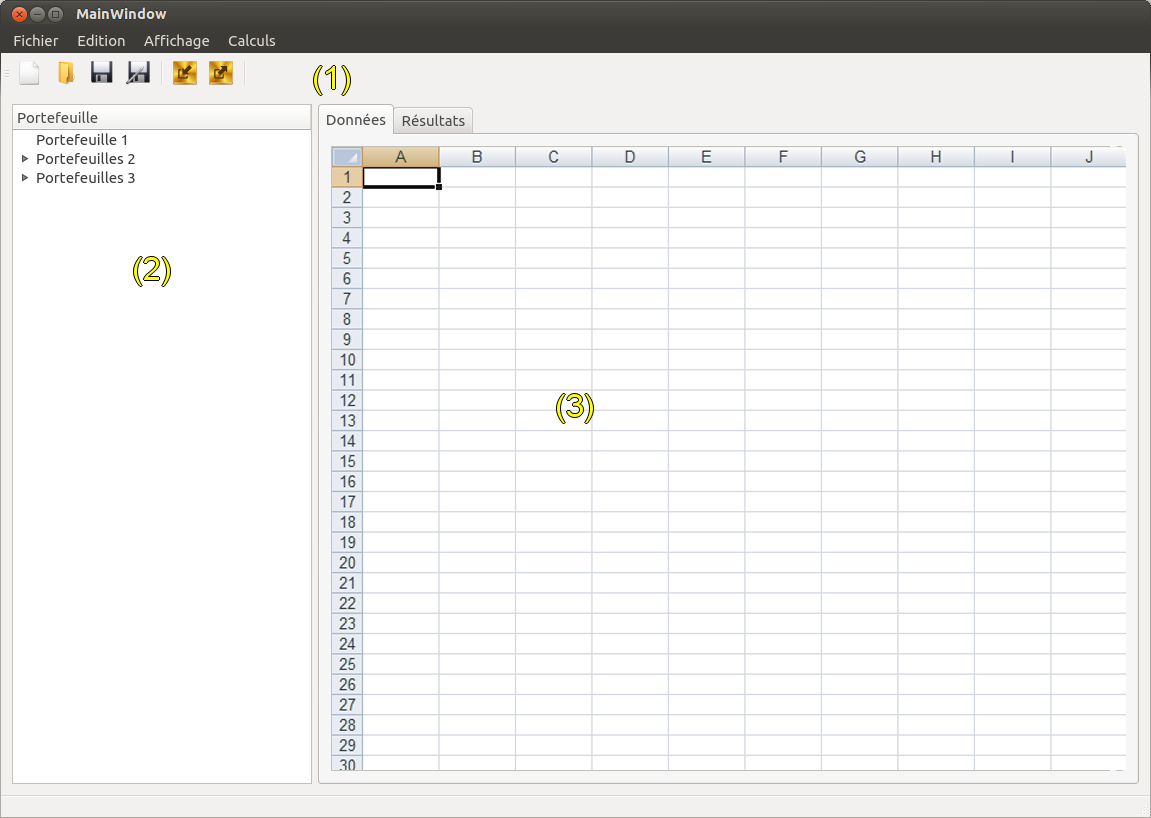
\includegraphics[width=400px]{logicielDonnees.png}
		\caption{Interface graphique : onglet données}
		\label{fig:interface}
		\begin{enumerate}
			\item Barre d’outils pour un accès rapide aux fonctionnalités les plus utilisées.
			\item Volet de selection des portefeuilles
			\item Affichage des données dans une grille 
		\end{enumerate}
	\end{figure}

	\begin{figure}[H]
		\center
		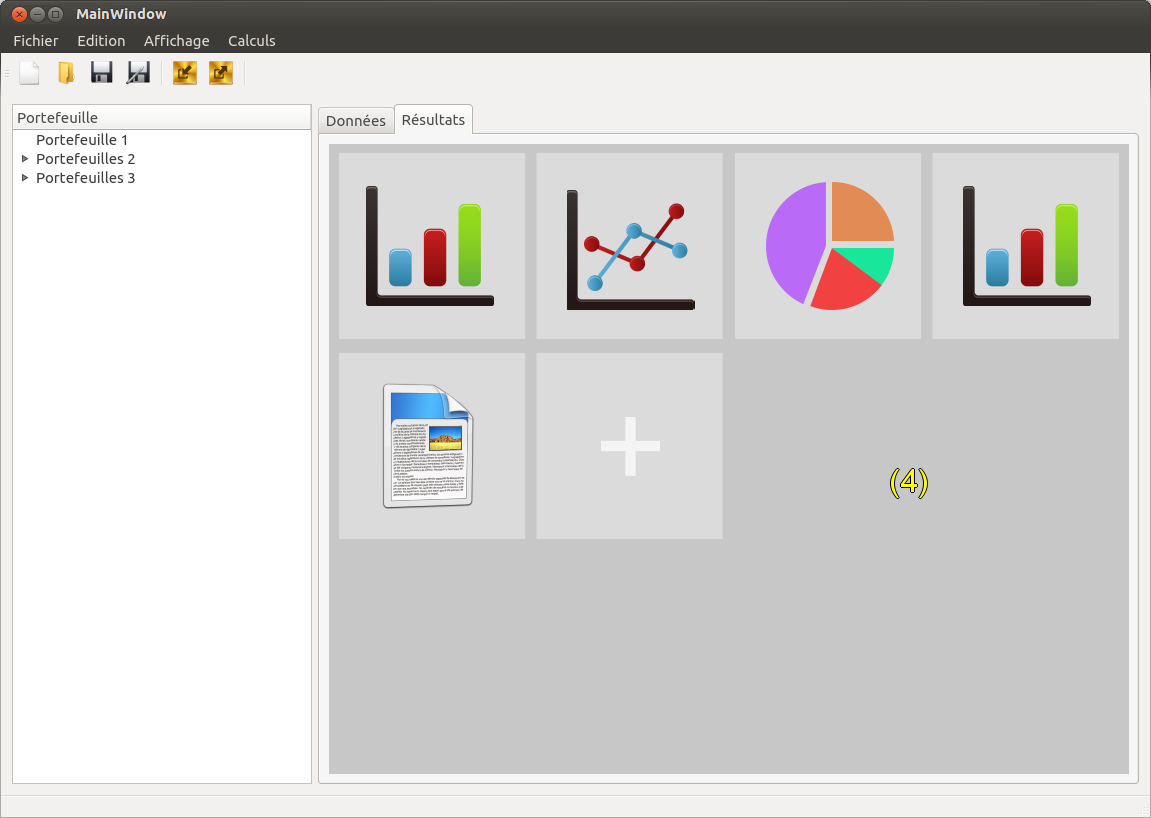
\includegraphics[width=400px]{logicielResultat.png}
		\caption{Interface graphique : onglet résultats}
		\label{fig:interface2}
		\begin{enumerate}
			\setcounter{enumi}{3} 
			\item Affichage des résultats
		\end{enumerate}
	\end{figure}



\section{Technologies utilisées}

\subsection{Excel}

Comme expliqué dans le rapport de pré-étude, de nombreuses fonctionnalités de notre logiciel sont celles d’un simple logiciel tableur.
Nous devons entre autres importer des données, les afficher sous formes de tableaux et de graphes ainsi que les exporter.

Nous pensions, au début (cf. rapport de pré-étude), intégrer Excel à notre logiciel pour implémenter ces fonctionnalités.
Cependant, il apparaît finalement que nous n'avons besoin que de quelques fonctions très simples.
Intégrer Excel semble donc disproportionné; nous développerons ces fonctionnalités à l'aide de Qt.


\subsection{Interfaçage avec R}

Nous allons avoir besoin du logiciel R pour effectuer certains calculs, notamment pour effectuer la modélisation GARCH.

Dans le rapport de pré-étude nous avions exposé différentes méthodes pour interfacer notre logiciel avec R.
Nous avons choisi d'utiliser la dernière exposée.
Celle-ci consiste à exécuter le code R directement depuis le code C++.
Les deux autres méthodes que nous avions décrites étaient moins utilisées et donc moins documentées.


\subsection{Qt pour l'interface graphique}

Nous avions réalisé la première maquette dans le rapport de pré-étude à l'aide de Qt.
Qt est un framework pour C++ qui offre des outils, entre autres, pour développer des interfaces graphiques.
Le framework contient aussi un environnement de développement facilitant la création d'interfaces graphiques.

Nous allons donc utiliser Qt et Qt Designer pour simplifier la création de l'interface graphique.
Dans le rapport de pré-étude, nous avions pensé utiliser Visual Studio comme outil de développement.
Cela était alors justifié par l'utilisation d'Excel pour nos opérations de tableur.
Nous pensons maintenant utiliser Qt Creator pour profiter de la meilleure intégration de Qt Designer.



\section{Architecture générale}

L'architecture de notre projet se découpe en différents modules assez simples.
Il y a une partie dédiée à l'affichage (GUI), une autre dédiée à la génération de graphiques, une aux calculs, une liée à la génération de rapports et une dernière qui contiendra les données de notre logiciel.
Nous utiliserons également deux outils extérieurs mentionnés précédemment : Qt pour la partie affichage et R pour la partie calcul.
Les différents modules sont ensuite dépendants les uns des autres en fonction des actions qu'ils effectuent.

\begin{figure}[H]
  \center
  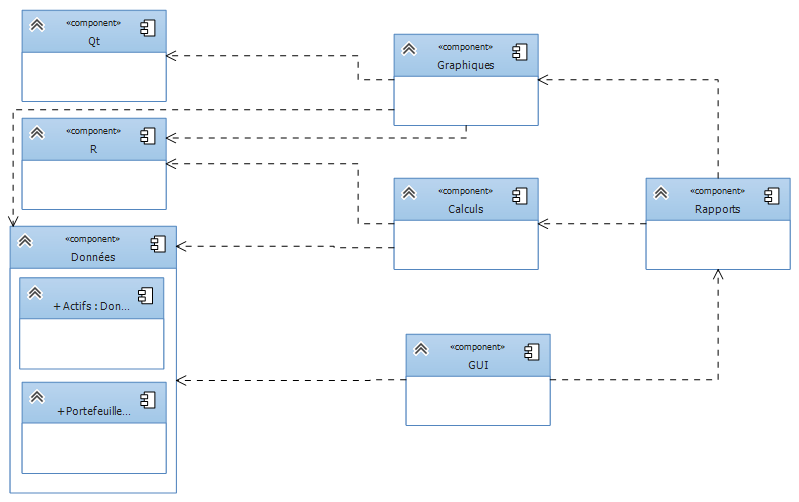
\includegraphics[width=1\textwidth]{ArchiGenerale.png}
  \caption{Architecture générale du projet}
\end{figure} 




\chapter{Conclusion}
Dans ce document nous avons défini les différentes fonctionnalités qui seront recherchées par une personne voulant manipuler des portefeuilles d’actifs et calculer la VaR sur ces derniers.
Le tout dans l'optique d'avoir un outil d'aide à la décision à la fois simple et efficace.
Les fonctionnalités suivantes seront implémentées : gestion des données, affichage des portefeuilles, calculs sur les portefeuilles et backtesting.

Lors de cette deuxième phase du projet, nous avons été amenés à réfléchir aux différentes fonctionnalités de notre application qui lui permettront de répondre à toutes les exigences des utilisateurs, mais aussi de se démarquer des solutions existantes sur le marché.
De plus, nous avons aussi choisi les différentes technologies que nous allons utiliser pour notre logiciel.

A la fin du projet, notre application devra implémenter toutes les fonctionnalités qui ont été décrites dans ce document.
La difficulté qui sera à surmonter durant le développement concerne les technologies utilisées.
Pour faire nos choix, nous avons réalisé différents tests et pris en compte les avis des personnes averties sur le sujet.
Cependant il n’est pas impossible que d’autres solutions se révèlent meilleures en cours de développement.

Cette étape de spécification étant terminée, nous allons pouvoir nous concentrer sur l’architecture globale de notre application, la planification et la répartition des tâches.


\end{document}